\subsection{Contrat vierge }
Le contrat vierge est un document Word généré automatiquement à partir des données contenues dans le fichier \texttt{MCC}.  
Il n’inclut pas encore les notes d’un·e étudiant·e, mais est entièrement adapté aux informations de l’année en cours (noms des UE, EC, etc.).  
Le code de génération n’a pas besoin d’être modifié chaque année : il s’adapte dynamiquement aux données du fichier \texttt{MCC}.

\vspace{0.5em}
\noindent Voici un aperçu de l’en-tête du contrat vierge :

\begin{figure}[ht]
    \centering
    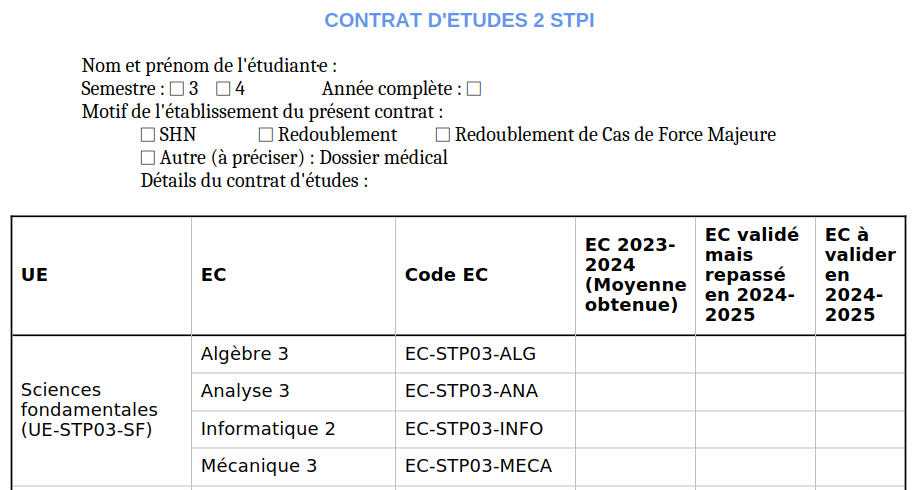
\includegraphics[width=\linewidth]{images/contrat_vierge.jpg}
    \caption{En-tête du contrat vierge}
    \label{contrat_vierge}
\end{figure}

\vspace{0.5em}
Le contrat contient également un espace dédié à la signature, situé à la fin du document.  
Cet espace est prévu pour :
\begin{itemize}
    \item la signature de l’étudiant·e précédée de la mention « lu et approuvé » ;
    \item la signature de la direction du département STPI ;
    \item l’apposition du cachet de l’établissement.
\end{itemize}

\begin{figure}[ht]
  \centering
  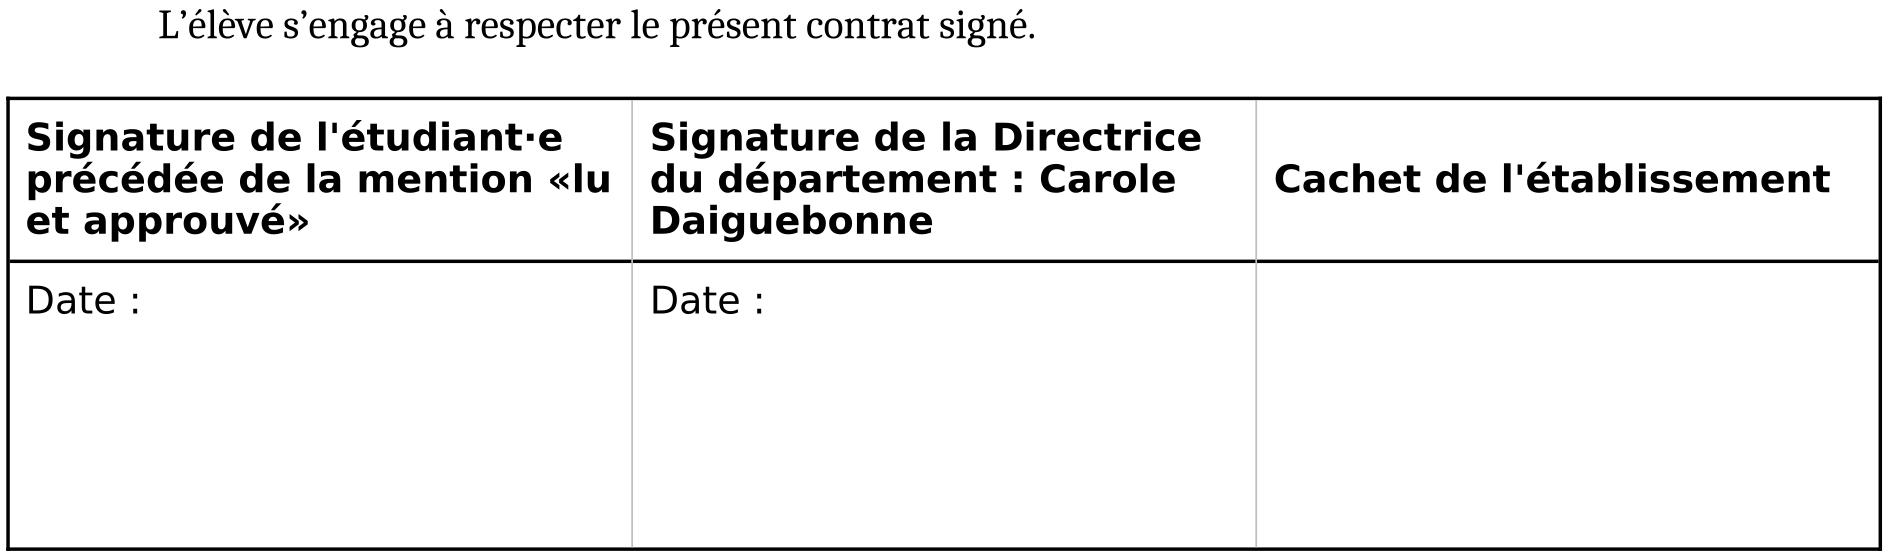
\includegraphics[width=\linewidth]{images/signature.jpg}
  \caption{Espace de signature du contrat}
  \label{signature}
\end{figure}


\subsection{Contrat avec notes }

Une fois les notes générées dans le fichier \texttt{jury.xlsx}, il est possible de générer automatiquement un contrat personnalisé pour chaque étudiant·e redoublant·e à partir de son identifiant.

\vspace{0.5em}
La génération repose sur la fonction \texttt{generation(id, doc)}, où \texttt{id} désigne l'identifiant de l’étudiant·e. Cette fonction :
\begin{itemize}
    \item extrait automatiquement le \textbf{nom} et le \textbf{prénom} de l’étudiant·e à partir de son identifiant ;
    \item insère ces informations en haut du contrat ;
    \item ajoute ses moyennes dans la colonne \textbf{« EC 2024-2025 (Moyenne obtenue) »} ;
    \item coche les EC dans la colonne \textbf{« EC à valider en 2024-2025 »} si :
        \begin{itemize}
            \item la moyenne de l’EC est strictement inférieure à 10 ou absente ;
            \item et l’UE correspondante est indiquée comme \textbf{non validée}.
        \end{itemize}
    \item intègre un tableau de signature à la fin du contrat.
\end{itemize}

